% ==========================================
% step05.tex
% ==========================================
\section[تعدیل هیستوگرام و مقایسه جامع]{بخش پنجم: تعدیل هیستوگرام و مقایسه نهایی}

\noindent
در بخش‌های پیشین، برای اصلاح کنتراست و روشنایی، نیازمند یافتن دستی یا محاسبه‌ی آماریِ پارامترها (مانند $a$، $b$ و $\gamma$) بودیم. تکنیک تعدیل هیستوگرام (\lr{Histogram Equalization}) یک روش غیرخطی و کاملاً خودکار است که بر پایه‌ی تابع توزیع تجمعی (\lr{CDF}) تصویر عمل می‌کند و هدف آن، دستیابی به توزیعی تخت (\lr{Uniform}) با استفاده از تمام ظرفیت دامنه‌ی دینامیکی (بازه ۰ تا ۲۵۵) است.

\begin{stepbox}
\field{۱. منطق ریاضی و پیاده‌سازی الگوریتم}{
این الگوریتم در سه گام آماری عمل می‌کند:
نخست، تابع چگالی احتمال (\lr{PDF}) برای هر سطح روشنایی $r_k$ محاسبه می‌شود: $p(r_k) = n_k / MN$. 
سپس، تابع توزیع تجمعی (\lr{CDF}) با جمع احتمالات به دست می‌آید. 
در نهایت، مقدار جدید پیکسل ($s_k$) از طریق نگاشت این توزیع به بالاترین سطح ممکن (برای تصویر ۸ بیتی $L-1 = 255$) محاسبه می‌گردد:
\[
s_k = T(r_k) = 255 \times \sum_{j=0}^{k} p(r_j)
\]
با توجه به ماهیت کاملاً استانداردِ این عملیات، استفاده از تابع \texttt{cv2.equalizeHist} در کتابخانه‌ی \lr{OpenCV} بهینه‌ترین روش پیاده‌سازی آن محسوب می‌شود.
}
\end{stepbox}

\begin{codebox}[پیاده‌سازی خودکار تعدیل هیستوگرام]
\begin{lstlisting}[language=Python]
import cv2

# Apply Global Histogram Equalization directly using OpenCV
I_DI_eq = cv2.equalizeHist(I_DI)
I_BI_eq = cv2.equalizeHist(I_BI)
\end{lstlisting}
\end{codebox}

\begin{figure}[htbp]
\centering
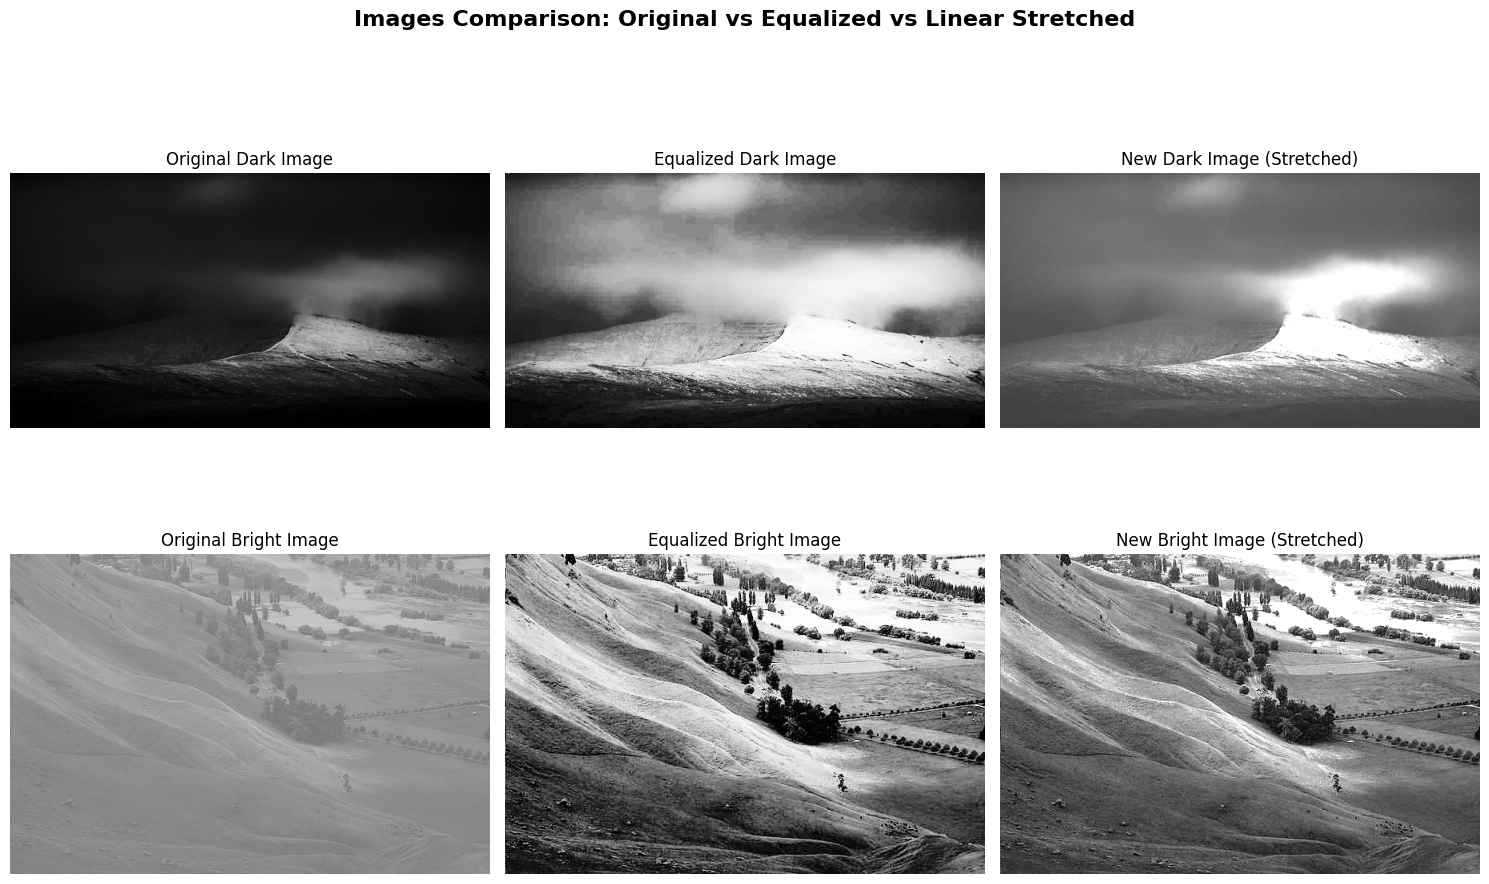
\includegraphics[width=\textwidth]{images/image_068277.png}
\caption{مقایسه بصری خروجی‌ها. ستون چپ: تصاویر خام، ستون وسط: خروجی تعدیل هیستوگرام، ستون راست: خروجی انتقال افاین (بخش ۳). به تقویت بیش از حد نویز در آسمان \texttt{DarkImage} در روش \lr{Equalization} دقت کنید.}
\label{fig:comparison_visual}
\end{figure}

\newpage
\begin{stepbox}
\field{۲. تحلیل نتایج بصری و تفاوت با انتقال خطی افاین}{
با مقایسه‌ی خروجی‌های تعدیل هیستوگرام و انتقال افاین ($a \times I + b$)، تفاوت ماهیت این دو روش کاملاً آشکار می‌شود:
\begin{itemize}[leftmargin=*]
    \item \textbf{در تصویر \texttt{BrightImage}:} تعدیل هیستوگرام عملکردی خیره‌کننده داشته است. بافت‌های پیچیده‌ی روی تپه‌ها و دشت‌ها، به دلیل توزیع شدنِ قدرتمندِ پیکسل‌ها در سراسر بازه، با کنتراستِ موضعیِ بسیار بالایی نمایان شده‌اند.
    \item \textbf{در تصویر \texttt{DarkImage}:} نقطه ضعف اصلی روشِ سراسریِ تعدیل هیستوگرام (\lr{Global HE}) در اینجا خودنمایی می‌کند. از آنجا که بخش عظیمی از تصویر را آسمانِ تاریک تشکیل داده است، الگوریتم برای تخت کردن هیستوگرام، فاصله‌ی نوریِ این پیکسل‌ها را به شدت کشیده است. این کار باعث شده نویزهایِ پنهانِ سنسور به شدت تقویت شده و آسمان حالتی دانه‌دانه و مصنوعی پیدا کند. در مقابل، روش خطی افاین (تصویر سمت راست) اگرچه کنتراست پایین‌تری دارد، اما خروجی بسیار طبیعی‌تری ارائه کرده است.
\end{itemize}
}
\end{stepbox}

\begin{figure}[htbp]
\centering
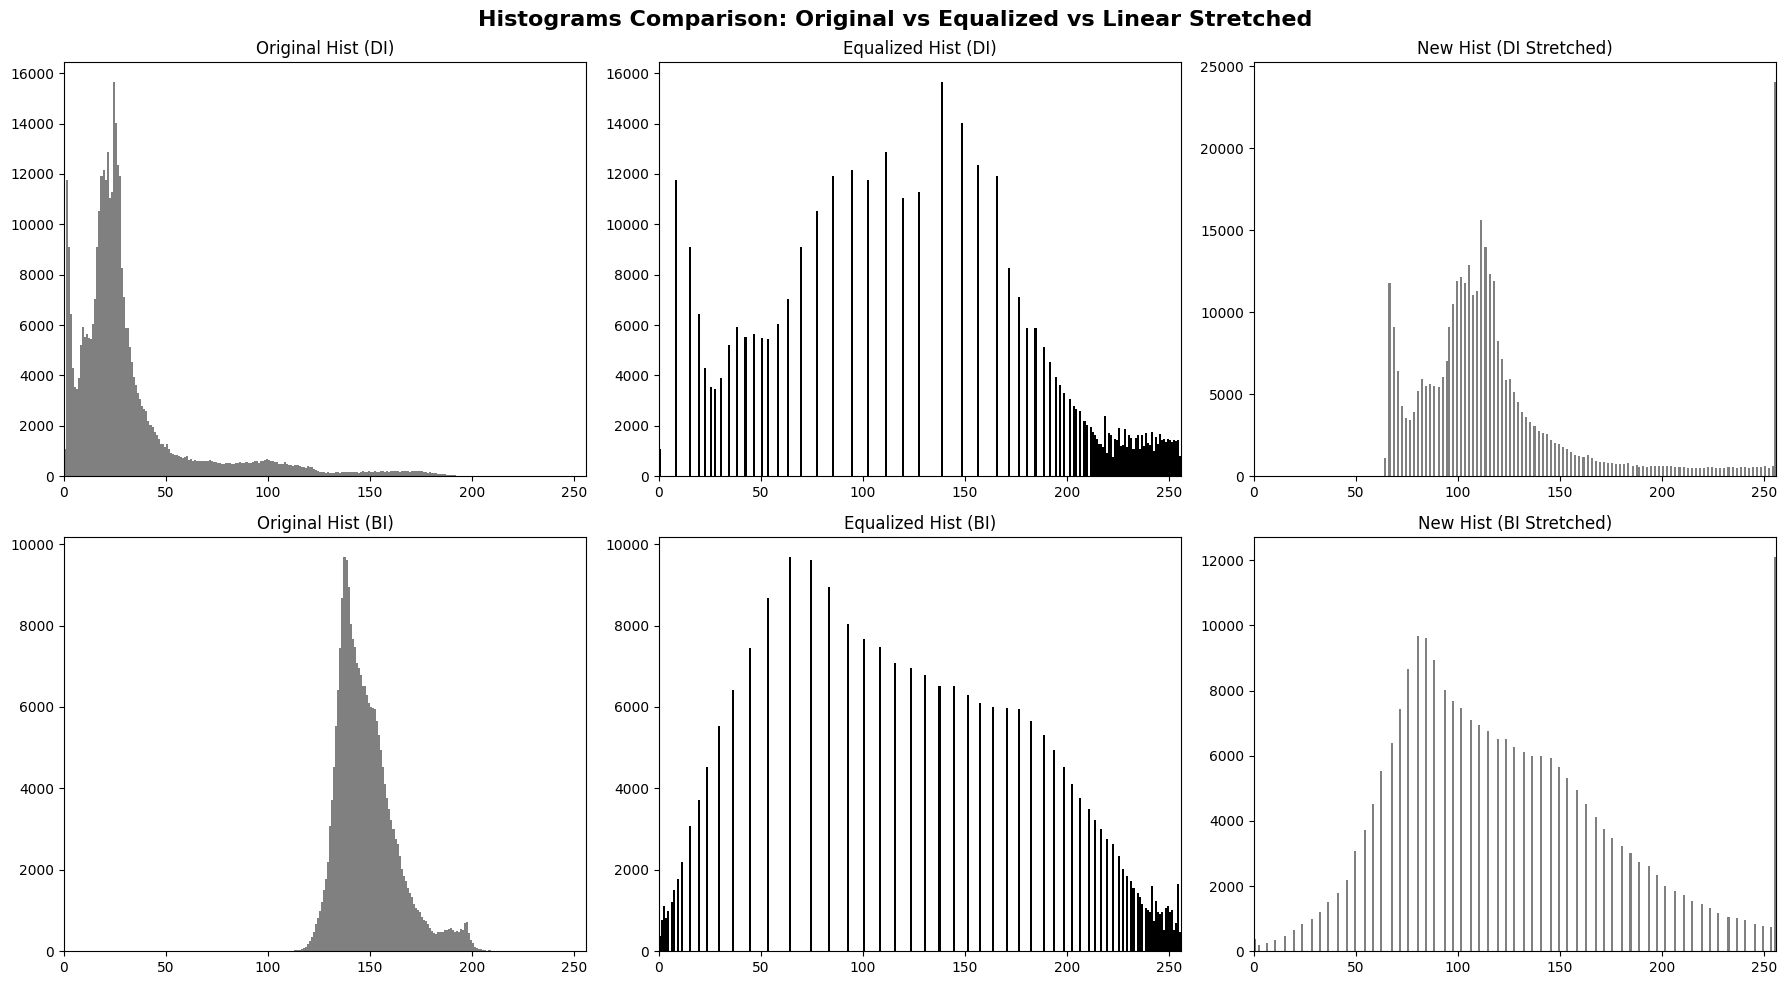
\includegraphics[width=\textwidth]{images/image_068291.png}
\caption{مقایسه هیستوگرام‌ها. گپ‌ها (فواصل خالی) در هیستوگرام‌های میانی به وضوح نشان‌دهنده ماهیت گسسته الگوریتم تعدیل هیستوگرام دیجیتال هستند.}
\label{fig:comparison_hist}
\end{figure}

\begin{notebox}[تحلیل هیستوگرام و پدیده \lr{Gaps}]
با دقت در هیستوگرام‌های تعدیل‌شده (ستون وسط)، مشاهده می‌شود که برخلاف حالت پیوسته در ریاضیات، هیستوگرام خروجی کاملاً تخت نیست و دارای شانه و فواصل خالی (\lr{Gaps}) متعددی است. دلیل این امر ماهیت گسسته‌ی (\lr{Discrete}) تصاویر دیجیتال است؛ الگوریتم نمی‌تواند پیکسل‌هایی که در مبدا مقدار یکسانی دارند را در مقادیر متفاوتی در مقصد توزیع کند، در نتیجه پرش‌هایی در هیستوگرام ایجاد می‌شود که ویژگی ذاتی این روش در تصاویر گسسته است.
\end{notebox}

\begin{tipbox}[جمع‌بندی و نتیجه‌گیری نهایی تمرین]
بررسی جامع عملگرهای نقطه‌ای نشان داد که هیچ راه‌حلِ جهان‌شمولی برای بهبود کیفیت تمام تصاویر وجود ندارد. عملگرهای خطی ($a \times I + b$) کنترل دقیقی به کاربر می‌دهند اما نیازمند تنظیم پارامتر هستند. توابع توانی (گاما) برای حفظ کیفیت نواحیِ حدی عالی‌اند و تعدیل هیستوگرام ابزاری قدرتمند و خودکار برای بیشینه‌سازی کنتراست سراسری است، به شرط آنکه مراقب تقویت نویزهای پس‌زمینه باشیم.
\end{tipbox}